\section{Umsetzungskonzept}
Die Grundidee für die Umsetzung der Zebrastreifen Erkennung lässt sich in folgenden Punkten zusammenfassen:
\begin{enumerate}
	\item Download der Strassen- und Zebrastreifenkoordinaten
	\item Download von Orthofotos auf Open Street Map Zoomstufe 19
	\item Anfertigen von einheitlichen Bildern entlang den Strassen
	\item Zebrastreifenerkennung mithilfe des Convnets
	\item Vergleich bestehende Zebrastreifen mit neu gefundenen
	\item Parallelisierung des Erkennungsprozesses
	\item Daten in eine Maproulette Challenge umwandeln
\end{enumerate}

\subsection{Open Street Map Anbindung}
Um Daten von Open Street Map zu erhalten, kann man eine Open Street Map Web API ansprechen. Mapquest\footnote{\url{http://open.mapquestapi.com/xapi/}} stellt eine solche Open Street Map API zur Verfügung. Mit dieser Schnittstelle lassen sich via HTTP GET Abfragen starten. Eine Bounding Box und die entsprechenden Open Street Map Tags dienen als Input. Man erhält danach alle Daten in einem einfach zu interpretierenden XML Format. Mit der gleichen Abfrage lassen sich sogar Zebrastreifen und Strassen gleichzeitig herunterladen.

\begin{figure}[H]
	\centering
	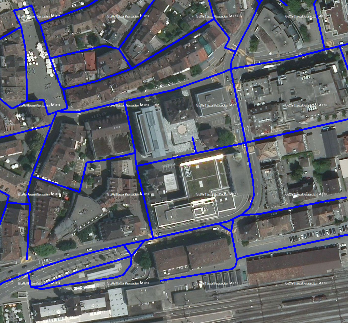
\includegraphics{images/Strassen_Rapperswil.png}
	\caption{Eingezeichnete Strassen in Rapperswil}
\end{figure}


\subsection{Bing Anbindung}
Um an die Orthofotos zu kommen, gab es zu Beginn des Projektes mehrere Lösungen:
\begin{enumerate}
	\item Offizielle Microsoft Bing REST Service
	\item Direkter Download über Bing Maps
	\item Benutzung der Orthofotos von der HSR
\end{enumerate}

Als aller erstes haben wir versucht, die Orthosfotos über den offizielle Microsoft Bing REST Service\footnote{\url{https://msdn.microsoft.com/en-us/library/ff701713.aspx}} zu download. Jedoch beschränkt Microsoft den API Zugriff auf 50'000 Transaktionen pro Tag und 125'000 Transaktionen pro Jahr, was uns bei geschätzten 7 Millionen Tiles in der Schweiz nicht reichen würde.

Nachdem diesem ersten Versuch sind wir auf den direkten Download der Othosfotos umgestiegen. Wenn man mit dem Internet Browser auf Bing Maps zugreift, werden die Tiles mithilfe von Javascript von den Bing Servern geladen. Microsoft benutzt das Quadtree\footnote{\url{https://msdn.microsoft.com/en-us/library/bb259689.aspx}} Format, um die entsprechenden Tiles anzusprechen. Mithilfe des Projekts Tiles à la Google Maps\footnote{\url{http://www.maptiler.org/google-maps-coordinates-tile-bounds-projection/}} und der dort zur Verfügung gestellten Python Library, können wir Bounding Boxen in Quadtrees umwandeln.

Die Orthofotos, welche im Besitz der HSR sind und die nur Schweiz umfassen, wären die letzte Lösung gewesen, wenn die anderen Möglichkeiten versagt hätten.

\subsection{Zebrastreifenvergleich}
\subsection{Parallelisierung}
\subsection{Maproulette Challenge}
